%Version 2.1 April 2023
% See section 11 of the User Manual for version history
%
%%%%%%%%%%%%%%%%%%%%%%%%%%%%%%%%%%%%%%%%%%%%%%%%%%%%%%%%%%%%%%%%%%%%%%
%%                                                                 %%
%% Please do not use \input{...} to include other tex files.       %%
%% Submit your LaTeX manuscript as one .tex document.              %%
%%                                                                 %%
%% All additional figures and files should be attached             %%
%% separately and not embedded in the \TeX\ document itself.       %%
%%                                                                 %%
%%%%%%%%%%%%%%%%%%%%%%%%%%%%%%%%%%%%%%%%%%%%%%%%%%%%%%%%%%%%%%%%%%%%%

\documentclass[sn-basic,pdflatex]{sn-jnl}

%%%% Standard Packages
%%<additional latex packages if required can be included here>

\usepackage{graphicx}%
\usepackage{multirow}%
\usepackage{amsmath,amssymb,amsfonts}%
\usepackage{amsthm}%
\usepackage{mathrsfs}%
\usepackage[title]{appendix}%
\usepackage{xcolor}%
\usepackage{textcomp}%
\usepackage{manyfoot}%
\usepackage{booktabs}%
\usepackage{algorithm}%
\usepackage{algorithmicx}%
\usepackage{algpseudocode}%
\usepackage{listings}%
%%%%

%%%%%=============================================================================%%%%
%%%%  Remarks: This template is provided to aid authors with the preparation
%%%%  of original research articles intended for submission to journals published
%%%%  by Springer Nature. The guidance has been prepared in partnership with
%%%%  production teams to conform to Springer Nature technical requirements.
%%%%  Editorial and presentation requirements differ among journal portfolios and
%%%%  research disciplines. You may find sections in this template are irrelevant
%%%%  to your work and are empowered to omit any such section if allowed by the
%%%%  journal you intend to submit to. The submission guidelines and policies
%%%%  of the journal take precedence. A detailed User Manual is available in the
%%%%  template package for technical guidance.
%%%%%=============================================================================%%%%

%% Per the spinger doc, new theorem styles can be included using built in style, 
%% but it seems the don't work so commented below
%\theoremstyle{thmstyleone}%
\newtheorem{theorem}{Theorem}%  meant for continuous numbers
%%\newtheorem{theorem}{Theorem}[section]% meant for sectionwise numbers
%% optional argument [theorem] produces theorem numbering sequence instead of independent numbers for Proposition
\newtheorem{proposition}[theorem]{Proposition}%
%%\newtheorem{proposition}{Proposition}% to get separate numbers for theorem and proposition etc.

%% \theoremstyle{thmstyletwo}%
\theoremstyle{remark}
\newtheorem{example}{Example}%
\newtheorem{remark}{Remark}%

%% \theoremstyle{thmstylethree}%
\theoremstyle{definition}
\newtheorem{definition}{Definition}%



\raggedbottom




% tightlist command for lists without linebreak
\providecommand{\tightlist}{%
  \setlength{\itemsep}{0pt}\setlength{\parskip}{0pt}}





\begin{document}


\title[Lab Notebook]{Ordinal Pattern Analysis for Early Bearing Fault
Detection and Classification in Rotating Machinery}

%%=============================================================%%
%% Prefix	-> \pfx{Dr}
%% GivenName	-> \fnm{Joergen W.}
%% Particle	-> \spfx{van der} -> surname prefix
%% FamilyName	-> \sur{Ploeg}
%% Suffix	-> \sfx{IV}
%% NatureName	-> \tanm{Poet Laureate} -> Title after name
%% Degrees	-> \dgr{MSc, PhD}
%% \author*[1,2]{\pfx{Dr} \fnm{Joergen W.} \spfx{van der} \sur{Ploeg} \sfx{IV} \tanm{Poet Laureate}
%%                 \dgr{MSc, PhD}}\email{iauthor@gmail.com}
%%=============================================================%%

\author*[1]{\fnm{Rasika} \sur{Dilhani} \dgr{MSc}}\email{\href{mailto:rasika.dilhani@vuw.ac.nz}{\nolinkurl{rasika.dilhani@vuw.ac.nz}}}

\author[1,2]{\fnm{Keila} \sur{Author} }

\author[1]{\fnm{Alejandro} \sur{Author} }



  \affil*[1]{\orgdiv{School of Mathematics and
Statistics}, \orgname{Victoria University of
Wellington}, \orgaddress{\city{Wellington}, \country{New
Zealand}, \postcode{6012}, \state{}, \street{}}}
  \affil*[2]{\orgname{Other Organisation}}

\abstract{\textbf{Purpose}: The abstract serves both as a general
introduction to the topic and as a brief, non-technical summary of the
main results and their implications. The abstract must not include
subheadings (unless expressly permitted in the journal's Instructions to
Authors), equations or citations. As a guide the abstract should not
exceed 200 words. Most journals do not set a hard limit however authors
are advised to check the author instructions for the journal they are
submitting to.

\textbf{Methods:} The abstract serves both as a general introduction to
the topic and as a brief, non-technical summary of the main results and
their implications. The abstract must not include subheadings (unless
expressly permitted in the journal's Instructions to Authors), equations
or citations. As a guide the abstract should not exceed 200 words. Most
journals do not set a hard limit however authors are advised to check
the author instructions for the journal they are submitting to.

\textbf{Results:} The abstract serves both as a general introduction to
the topic and as a brief, non-technical summary of the main results and
their implications. The abstract must not include subheadings (unless
expressly permitted in the journal's Instructions to Authors), equations
or citations. As a guide the abstract should not exceed 200 words. Most
journals do not set a hard limit however authors are advised to check
the author instructions for the journal they are submitting to.

\textbf{Conclusion:} The abstract serves both as a general introduction
to the topic and as a brief, non-technical summary of the main results
and their implications. The abstract must not include subheadings
(unless expressly permitted in the journal's Instructions to Authors),
equations or citations. As a guide the abstract should not exceed 200
words. Most journals do not set a hard limit however authors are advised
to check the author instructions for the journal they are submitting
to.\}}

\keywords{key, dictionary, word}


\pacs[JEL Classification]{D8, H51}
\pacs[MSC Classification]{35A01, 65L10}

\maketitle

\section{Introduction}\label{sec1}

Bearings are critical components in rotating machinery, yet their
demanding operating conditions involving high loads and impacts often
lead to various faults. These faults can result in significant downtime,
costly maintenance, and even complete machine failure. Therefore, early
and accurate detection and classification of bearing faults are
essential for ensuring operational reliability and minimizing
maintenance expenses.

Traditional fault detection methods primarily rely on analyzing physical
parameters and trends using techniques such as vibration analysis,
thermal monitoring, and current signature analysis. While these methods
have proven effective, they can be susceptible to noise and often
require substantial computational resources. Ordinal pattern analysis
has emerged as a promising alternative, offering a robust and
computationally efficient approach for analyzing time series data.

At its core, ordinal pattern analysis involves transforming continuous
time series data into a sequence of ordinal patterns that represent the
order relationships among data points within a given time window. This
approach effectively captures the fundamental dynamics of the signal in
a manner that is inherently robust to noise and distortions. By
analyzing these patterns, it becomes possible to identify subtle changes
in system behavior that may indicate the presence of a fault.

This study investigates the application of ordinal pattern analysis for
early detection and classification of bearing faults, focusing on common
fault types such as ball, outer race, and inner race defects. Using a
publicly available dataset from the Case Western Reserve University
Bearing Data Center, we will demonstrate the effectiveness of ordinal
patterns in distinguishing between healthy and faulty bearing
conditions.

Our research will explore the advantages of ordinal pattern analysis in
detecting changes in system dynamics associated with faults. By
identifying alterations in the frequency and recurrence of specific
temporal patterns, this technique can reveal subtle indicators of
developing faults. Furthermore, unlike some traditional methods limited
to linear systems, ordinal pattern analysis can effectively detect
faults in complex, non-linear systems, broadening its applicability.

This study will also compare the performance of ordinal pattern analysis
with traditional fault detection techniques, evaluating metrics such as
accuracy, sensitivity, and computational efficiency. While traditional
methods often rely on specialized sensors and data acquisition systems,
ordinal pattern analysis can potentially achieve comparable results
using simpler time series data, highlighting its potential for wider
adoption. Additionally, we will investigate the sensitivity of ordinal
pattern analysis to subtle changes in system dynamics, particularly
within complex systems, where its strengths may be most pronounced.

We aim to establish ordinal pattern analysis as a viable and
advantageous tool for bearing fault diagnosis, contributing to the
advancement of predictive maintenance technologies and promoting more
efficient and reliable operation of rotating machinery.

\section{Ordinal Patterns}\label{sec2}

\section{Literature Review}\label{sec3}

The authors of \citep{WOS:000312724900101} present an enhanced method
for detecting bearing faults by leveraging high frequency resonance,
which improves the accuracy and reliability of fault diagnosis in
mechanical systems. The study demonstrates that the improved technique
effectively identifies early-stage bearing defects, providing a
significant advancement over traditional diagnostic methods. The paper
\citep{WOS:000301688000008} introduces a novel method for fault
detection that utilizes an adaptive rank-order morphological filter to
classify patterns in one-dimensional signals. This approach enhances the
accuracy and robustness of fault diagnosis by effectively filtering and
identifying signal anomalies. Moreover, in the literature, authors in
\citep{WOS:000303039300034} proposes a method for early fault detection
in machines by analyzing truncated vibration signals using Shannon
wavelet spectrum analysis. This technique enhances the identification of
incipient faults, improving the predictive maintenance of machinery. A
prototype FPGA implementation leverages machine learning to convert
analog signals into succinct feature representations, using an
event-based approach to enhance the efficiency and accuracy of signal
processing in various applications \citep{WOS:000345844100102}. A
dedicated hierarchy of neural networks is applied to assess bearing
degradation, improving the accuracy and reliability of diagnosing the
condition and remaining useful life of bearings in machinery was
discusses in the paper \citep{WOS:000396580800080}. In the paper
\citep{WOS:000320835800016}, the fault diagnosis of rolling bearings is
enhanced by combining multifractal detrended fluctuation analysis with
the Mahalanobis distance criterion, enhancing diagnostic accuracy and
providing effective, validated techniques for early fault detection in
industrial applications. Another interesting research work in the paper
\citep{WOS:000360994300029} presents a diagnostic method for rolling
element bearings based on the theory of active perception, which
involves analyzing dynamic interactions between the bearing and its
environment. Significant findings include the method's ability to
accurately assess bearing condition by incorporating perceptual cues and
responses, thus improving fault detection and predictive maintenance
strategies. With the research implement of \citep{WOS:000343577703075}
introduces a fault diagnosis method for rolling element bearings that
employs Empirical Mode Decomposition (EMD) combined with Discrete
Fourier Domain Analysis (DFDA). The method effectively isolates and
analyzes fault-related features in vibration signals, leading to
improved accuracy and reliability in diagnosing bearing conditions. A
signal-based triangular structuring element for mathematical
morphological analysis, applying this approach to enhance fault
diagnosis in rolling element bearings by effectively processing and
interpreting vibration signal features were discussed in the
\citep{WOS:000334316700001}. Moreover, a hybrid CEEMD-EMD approach for
fault detection in rolling bearings, which combines Complete Ensemble
Empirical Mode Decomposition with Noise (CEEMD) and traditional
Empirical Mode Decomposition (EMD) to improve the accuracy of vibration
signal analysis and enhance fault detection capabilities have improved
in the paper \citep{WOS:000412752200052}. Authors in the paper
\citep{WOS:000335959500009} proposes a bearing fault detection method
that utilizes compressive measurements of vibration signals to
efficiently identify faults, enhancing diagnostic accuracy while
reducing the data processing burden. A novel feature extraction method
based on the crossover characteristics of nonlinear data, applying it to
improve fault diagnosis in rotary machinery by effectively identifying
critical patterns in complex signal data has been studied with
\citep{WOS:000338603900013}. The studies demonstrate that
Self-Organizing Maps (SOMs) effectively diagnose motor bearing faults by
classifying complex vibration data, while methods based on fast nonlocal
means and envelope spectra improve fault diagnosis accuracy.
Additionally, a low-dimensional compressed measurement approach enhances
fault detection efficiency, and a smoothness index-guided Bayesian
inference technique offers precise identification of various bearing
faults by analyzing anti-symmetric real Laplace wavelet parameters
\citep[\citet{WOS:000348309400067}, \citet{WOS:000354607100016},
\citet{WOS:000350998800016}]{WOS:000380543400119}. Recent research has
focused on advanced techniques for bearing fault diagnosis using
vibration signals. Statistical locally linear embedding has been
proposed as an effective method for dimensionality reduction and feature
extraction, outperforming traditional approaches like PCA and LDA
\citep{WOS:000361788200068}.

\section{Results}\label{sec4}

Sample body text. Sample body text. Sample body text. Sample body text.
Sample body text. Sample body text. Sample body text. Sample body text.

\section{This is an example for first level head---section
head}\label{sec5}

\subsection{This is an example for second level head---subsection
head}\label{subsec2}

\subsubsection{This is an example for third level head---subsubsection
head}\label{subsubsec2}

Sample body text. Sample body text. Sample body text. Sample body text.
Sample body text. Sample body text. Sample body text.

\section{Equations}\label{sec6}

Equations in \LaTeX~can either be inline or on-a-line by itself
(``display equations''). For inline equations use the \texttt{\$...\$}
commands. E.g.: The equation \(H\psi = E \psi\) is written via the
command \texttt{\$H\ \textbackslash{}psi\ =\ E\ \textbackslash{}psi\$}.

For display equations (with auto generated equation numbers) one can use
the equation or align environments:

\begin{equation}
\|\tilde{X}(k)\|^2 \leq\frac{\sum\limits_{i=1}^{p}\left\|\tilde{Y}_i(k)\right\|^2+\sum\limits_{j=1}^{q}\left\|\tilde{Z}_j(k)\right\|^2 }{p+q}.\label{eq1}
\end{equation}

where, \begin{align}
D_\mu &=  \partial_\mu - ig \frac{\lambda^a}{2} A^a_\mu \nonumber \\
F^a_{\mu\nu} &= \partial_\mu A^a_\nu - \partial_\nu A^a_\mu + g f^{abc} A^b_\mu A^a_\nu \label{eq2}
\end{align}

Notice the use of \texttt{\textbackslash{}nonumber} in the align
environment at the end of each line, except the last, so as not to
produce equation numbers on lines where no equation numbers are
required. The \texttt{\textbackslash{}label\{\}} command should only be
used at the last line of an align environment where
\texttt{\textbackslash{}nonumber} is not used.

\begin{equation}
Y_\infty = \left( \frac{m}{\textrm{GeV}} \right)^{-3}
    \left[ 1 + \frac{3 \ln(m/\textrm{GeV})}{15}
    + \frac{\ln(c_2/5)}{15} \right]
\end{equation}

The class file also supports the use of
\texttt{\textbackslash{}mathbb\{\}},
\texttt{\textbackslash{}mathscr\{\}} and
\texttt{\textbackslash{}mathcal\{\}} commands. As such
\texttt{\textbackslash{}mathbb\{R\}},
\texttt{\textbackslash{}mathscr\{R\}} and
\texttt{\textbackslash{}mathcal\{R\}} produces \(\mathbb{R}\),
\(\mathscr{R}\) and \(\mathcal{R}\) respectively (refer
Subsubsection~\ref{subsubsec2}).

\section{Tables}\label{sec7}

Tables can be inserted via the normal \texttt{knitr::kable()} function
or other table-generating packages.

\begin{table}

\caption{\label{tab:tab1}Caption text}
\centering
\begin{tabular}[t]{r|r}
\hline
temperature & pressure\\
\hline
0 & 0.0002\\
\hline
20 & 0.0012\\
\hline
40 & 0.0060\\
\hline
60 & 0.0300\\
\hline
80 & 0.0900\\
\hline
100 & 0.2700\\
\hline
\end{tabular}
\end{table}

Tables can also be inserted via the normal table and tabular
environment. To put footnotes inside tables you should use
\texttt{\textbackslash{}footnotetext{[}{]}\{...\}} tag. The footnote
appears just below the table itself (refer
Tables\textasciitilde{}\ref{tab1} and \ref{tab2}). For the corresponding
footnotemark use \texttt{\textbackslash{}footnotemark{[}...{]}}

\begin{table}[h]
\caption{Caption text}\label{tab1}%
\begin{tabular}{@{}llll@{}}
\toprule
Column 1 & Column 2  & Column 3 & Column 4\\
\midrule
row 1    & data 1   & data 2  & data 3  \\
row 2    & data 4   & data 5\footnotemark[1]  & data 6  \\
row 3    & data 7   & data 8  & data 9\footnotemark[2]  \\
\botrule
\end{tabular}
\footnotetext{Source: This is an example of table footnote. This is an example of table footnote.}
\footnotetext[1]{Example for a first table footnote. This is an example of table footnote.}
\footnotetext[2]{Example for a second table footnote. This is an example of table footnote.}
\end{table}

\noindent The input format for the above table is as follows:

\begin{verbatim}
\begin{table}[<placement-specifier>]
\caption{<table-caption>}\label{<table-label>}%
\begin{tabular}{@{}llll@{}}
\toprule
Column 1 & Column 2 & Column 3 & Column 4\\
\midrule
row 1 & data 1 & data 2  & data 3 \\
row 2 & data 4 & data 5\footnotemark[1] & data 6 \\
row 3 & data 7 & data 8  & data 9\footnotemark[2]\\
\botrule
\end{tabular}
\footnotetext{Source: This is an example of table footnote.
This is an example of table footnote.}
\footnotetext[1]{Example for a first table footnote.
This is an example of table footnote.}
\footnotetext[2]{Example for a second table footnote.
This is an example of table footnote.}
\end{table}
\end{verbatim}

\begin{table}[h]
\caption{Example of a lengthy table which is set to full textwidth}\label{tab2}
\begin{tabular*}{\textwidth}{@{\extracolsep\fill}lcccccc}
\toprule%
& \multicolumn{3}{@{}c@{}}{Element 1\footnotemark[1]} & \multicolumn{3}{@{}c@{}}{Element 2\footnotemark[2]} \\\cmidrule{2-4}\cmidrule{5-7}%
Project & Energy & $\sigma_{calc}$ & $\sigma_{expt}$ & Energy & $\sigma_{calc}$ & $\sigma_{expt}$ \\
\midrule
Element 3  & 990 A & 1168 & $1547\pm12$ & 780 A & 1166 & $1239\pm100$\\
Element 4  & 500 A & 961  & $922\pm10$  & 900 A & 1268 & $1092\pm40$\\
\botrule
\end{tabular*}
\footnotetext{Note: This is an example of table footnote. This is an example of table footnote this is an example of table footnote this is an example of~table footnote this is an example of table footnote.}
\footnotetext[1]{Example for a first table footnote.}
\footnotetext[2]{Example for a second table footnote.}
\end{table}

\vfill\eject

In case of double column layout, tables which do not fit in single
column width should be set to full text width. For this, you need to use
\texttt{\textbackslash{}begin\{table*\}} \texttt{...}
\texttt{\textbackslash{}end\{table*\}} instead of
\texttt{\textbackslash{}begin\{table\}} \texttt{...}
\texttt{\textbackslash{}end\{table\}} environment. Lengthy tables which
do not fit in textwidth should be set as rotated table. For this, you
need to use \texttt{\textbackslash{}begin\{sidewaystable\}} \texttt{...}
\texttt{\textbackslash{}end\{sidewaystable\}} instead of
\texttt{\textbackslash{}begin\{table*\}} \texttt{...}
\texttt{\textbackslash{}end\{table*\}} environment. This environment
puts tables rotated to single column width. For tables rotated to double
column width, use \texttt{\textbackslash{}begin\{sidewaystable*\}}
\texttt{...} \texttt{\textbackslash{}end\{sidewaystable*\}}.

\begin{sidewaystable}
\caption{Tables which are too long to fit, should be written using the "sidewaystable" environment as shown here}\label{tab3}
\begin{tabular*}{\textheight}{@{\extracolsep\fill}lcccccc}
\toprule%
& \multicolumn{3}{@{}c@{}}{Element 1\footnotemark[1]}& \multicolumn{3}{@{}c@{}}{Element\footnotemark[2]} \\\cmidrule{2-4}\cmidrule{5-7}%
Projectile & Energy & $\sigma_{calc}$ & $\sigma_{expt}$ & Energy & $\sigma_{calc}$ & $\sigma_{expt}$ \\
\midrule
Element 3 & 990 A & 1168 & $1547\pm12$ & 780 A & 1166 & $1239\pm100$ \\
Element 4 & 500 A & 961  & $922\pm10$  & 900 A & 1268 & $1092\pm40$ \\
Element 5 & 990 A & 1168 & $1547\pm12$ & 780 A & 1166 & $1239\pm100$ \\
Element 6 & 500 A & 961  & $922\pm10$  & 900 A & 1268 & $1092\pm40$ \\
\botrule
\end{tabular*}
\footnotetext{Note: This is an example of table footnote this is an example of table footnote this is an example of table footnote this is an example of~table footnote this is an example of table footnote.}
\footnotetext[1]{This is an example of table footnote.}
\end{sidewaystable}

\section{Figures}\label{sec6}

As per the \LaTeX~standards you need to use eps images for
\LaTeX~compilation and \texttt{pdf/jpg/png} images for \texttt{PDFLaTeX}
compilation. Use the \texttt{dev} knitr option to use the approrpate
format. This is one of the major difference between \LaTeX~and
\texttt{PDFLaTeX}. Each image should be from a single input .eps/vector
image file. Avoid using subfigures. The command for inserting images for
\LaTeX~and \texttt{PDFLaTeX} can be generalized. The package used to
insert images in \texttt{LaTeX/PDFLaTeX} is the graphicx package.
Figures can be inserted via the normal figure environment as shown in
the below example:

\begin{figure}
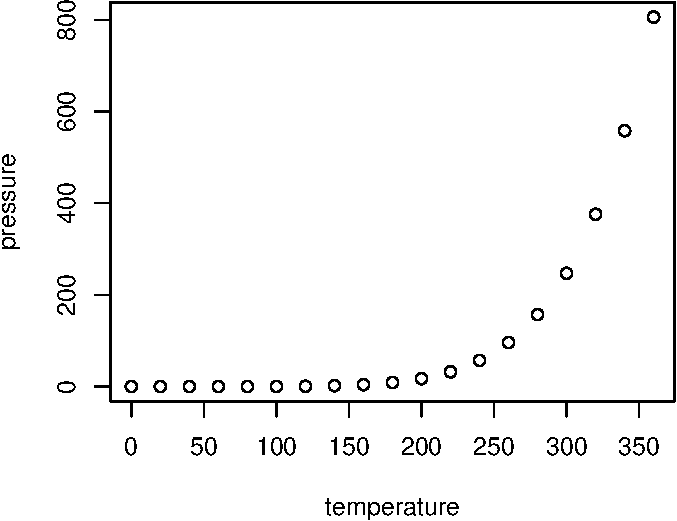
\includegraphics{Laboratory-Notebook_files/figure-latex/fig1-1} \caption{This is an example of a caption}\label{fig:fig1}
\end{figure}

\section{Algorithms, Program codes and Listings}\label{sec7}

Packages \texttt{algorithm}, \texttt{algorithmicx} and
\texttt{algpseudocode} are used for setting algorithms in \LaTeX~using
the format:

\begin{verbatim}
\begin{algorithm}
\caption{<alg-caption>}\label{<alg-label>}
\begin{algorithmic}[1]
. . .
\end{algorithmic}
\end{algorithm}
\end{verbatim}

You may refer above listed package documentations for more details
before setting \texttt{algorithm} environment. For program codes, the
``program'' package is required and the command to be used is
\texttt{\textbackslash{}begin\{program\}} \texttt{...}
\texttt{\textbackslash{}end\{program\}}. A fast exponentiation
procedure:

Similarly, for \texttt{listings}, use the \texttt{listings} package.
\texttt{\textbackslash{}begin\{lstlisting\}} \texttt{...}
\texttt{\textbackslash{}end\{lstlisting\}} is used to set environments
similar to \texttt{verbatim} environment. Refer to the
\texttt{lstlisting} package documentation for more details.

A fast exponentiation procedure:

\lstset{texcl=true,basicstyle=\small\sf,commentstyle=\small\rm,mathescape=true,escapeinside={(*}{*)}}
\begin{lstlisting}
begin
  for $i:=1$ to $10$ step $1$ do
      expt($2,i$);  
      newline() od                (*\textrm{Comments will be set flush to the right margin}*)
where
proc expt($x,n$) $\equiv$
  $z:=1$;
  do if $n=0$ then exit fi;
     do if odd($n$) then exit fi;                 
        comment: (*\textrm{This is a comment statement;}*)
        $n:=n/2$; $x:=x*x$ od;
     { $n>0$ };
     $n:=n-1$; $z:=z*x$ od;
  print($z$). 
end
\end{lstlisting}

\begin{algorithm}
\caption{Calculate $y = x^n$}\label{algo1}
\begin{algorithmic}[1]
\Require $n \geq 0 \vee x \neq 0$
\Ensure $y = x^n$ 
\State $y \Leftarrow 1$
\If{$n < 0$}\label{algln2}
        \State $X \Leftarrow 1 / x$
        \State $N \Leftarrow -n$
\Else
        \State $X \Leftarrow x$
        \State $N \Leftarrow n$
\EndIf
\While{$N \neq 0$}
        \If{$N$ is even}
            \State $X \Leftarrow X \times X$
            \State $N \Leftarrow N / 2$
        \Else[$N$ is odd]
            \State $y \Leftarrow y \times X$
            \State $N \Leftarrow N - 1$
        \EndIf
\EndWhile
\end{algorithmic}
\end{algorithm}

\begin{minipage}{\hsize}

\lstset{frame=single,framexleftmargin=-1pt,framexrightmargin=-17pt,framesep=12pt,linewidth=0.98\textwidth,language=pascal}

\begin{lstlisting}
for i:=maxint to 0 do begin \{ do nothing \} end; Write(`Case
insensitive'); Write(`Pascal keywords.');

\end{lstlisting}

\end{minipage}

\section{Cross referencing}\label{sec8}

Figures and tables are labeled with a prefix (fig or tab, respectively)
plus the chunk label. Other environments such as equation and align can
be labelled via the \texttt{\textbackslash{}label\{\#label\}} command
inside or just below the \texttt{\textbackslash{}caption\{\}} command.
You can then use the label for cross-reference. As an example, consider
the chunk label declared for Figure~\ref{fig:fig1} which is fig1. To
cross-reference it, use the command
\texttt{Figure\ \textbackslash{}ref\{fig:fig1\}}, for which it comes up
as ``Figure~\ref{fig:fig1}''.

To reference line numbers in an algorithm, consider the label declared
for the line number 2 of Algorithm~\ref{algo1} is
\texttt{\textbackslash{}label\{algln2\}}. To cross-reference it, use the
command \texttt{\textbackslash{}ref\{algln2\}} for which it comes up as
line~\ref{algln2} of Algorithm~\ref{algo1}.

\subsection{Details on reference citations}\label{subsec7}

For citations of references, use~\citet{bib1} or \citep{bib2}.

\section{Examples for theorem like environments}\label{sec10}

The documentclass for springer \texttt{sn-jnl.cls} contains 3 styling
that you can use to set new default for theorems and proofs type

\begin{description}
\item[\texttt{thmstyleone}]
Numbered, theorem head in bold font and theorem text in italic style
\item[\texttt{thmstyletwo}]
Numbered, theorem head in roman font and theorem text in italic style
\item[\texttt{thmstylethree}]
Numbered, theorem head in bold font and theorem text in roman style
\end{description}

For mathematics journals, theorem styles can be included as shown in the
following examples.

\begin{theorem}
Example theorem text. Example theorem text. Example theorem text.
Example theorem text. Example theorem text. Example theorem text.
Example theorem text. Example theorem text. Example theorem text.
Example theorem text. Example theorem text.

\end{theorem}

To add labels and subheadings, use LaTeX notation

\begin{theorem}[Theorem subhead]\label{thm1}
Example theorem text. Example theorem text. Example theorem text.
Example theorem text. Example theorem text. Example theorem text.
Example theorem text. Example theorem text. Example theorem text.
Example theorem text. Example theorem text.

\end{theorem}

Other environments are proposition, example, remark, definition, proof
and quote

Sample body text. Sample body text. Sample body text. Sample body text.
Sample body text. Sample body text. Sample body text. Sample body text.

\begin{proposition}
Example proposition text. Example proposition text. Example proposition
text. Example proposition text. Example proposition text. Example
proposition text. Example proposition text. Example proposition text.
Example proposition text. Example proposition text.

\end{proposition}

Sample body text. Sample body text. Sample body text. Sample body text.
Sample body text. Sample body text. Sample body text. Sample body text.

\begin{example}
Phasellus adipiscing semper elit. Proin fermentum massa ac quam. Sed
diam turpis, molestie vitae, placerat a, molestie nec, leo. Maecenas
lacinia. Nam ipsum ligula, eleifend at, accumsan nec, suscipit a, ipsum.
Morbi blandit ligula feugiat magna. Nunc eleifend consequat lorem.

\end{example}

Sample body text. Sample body text. Sample body text. Sample body text.
Sample body text. Sample body text. Sample body text. Sample body text.

\begin{remark}
Phasellus adipiscing semper elit. Proin fermentum massa ac quam. Sed
diam turpis, molestie vitae, placerat a, molestie nec, leo. Maecenas
lacinia. Nam ipsum ligula, eleifend at, accumsan nec, suscipit a, ipsum.
Morbi blandit ligula feugiat magna. Nunc eleifend consequat lorem.

\end{remark}

Sample body text. Sample body text. Sample body text. Sample body text.
Sample body text. Sample body text. Sample body text. Sample body text.

\begin{definition}[Definition sub head]
Example definition text. Example definition text. Example definition
text. Example definition text. Example definition text. Example
definition text. Example definition text. Example definition text.

\end{definition}

Additionally a predefined ``proof'' environment is available. This
prints a ``Proof'' head in italic font style and the ``body text'' in
roman font style with an open square at the end of each proof
environment.

\begin{proof}
Example for proof text. Example for proof text. Example for proof text.
Example for proof text. Example for proof text. Example for proof text.
Example for proof text. Example for proof text. Example for proof text.
Example for proof text.

\end{proof}

Sample body text. Sample body text. Sample body text. Sample body text.
Sample body text. Sample body text. Sample body text. Sample body text.

\section{Methods}\label{sec11}

Topical subheadings are allowed. Authors must ensure that their Methods
section includes adequate experimental and characterization data
necessary for others in the field to reproduce their work. Authors are
encouraged to include RIIDs where appropriate.

\textbf{Ethical approval declarations} (only required where applicable)
Any article reporting experiment/s carried out on
(i)\textasciitilde live vertebrate (or higher invertebrates),
(ii)\textasciitilde humans or (iii)\textasciitilde human samples must
include an unambiguous statement within the methods section that meets
the following requirements:

\begin{enumerate}
\def\labelenumi{\arabic{enumi}.}
\item
  Approval: a statement which confirms that all experimental protocols
  were approved by a named institutional and/or licensing committee.
  Please identify the approving body in the methods section
\item
  Accordance: a statement explicitly saying that the methods were
  carried out in accordance with the relevant guidelines and regulations
\item
  Informed consent (for experiments involving humans or human tissue
  samples): include a statement confirming that informed consent was
  obtained from all participants and/or their legal guardian/s
\end{enumerate}

If your manuscript includes potentially identifying patient/participant
information, or if it describes human transplantation research, or if it
reports results of a clinical trial then additional information will be
required. Please visit
(\url{https://www.nature.com/nature-research/editorial-policies}) for
Nature Portfolio journals,
(\url{https://www.springer.com/gp/authors-editors/journal-author/journal-author-helpdesk/publishing-ethics/14214})
for Springer Nature journals, or
(\url{https://www.biomedcentral.com/getpublished/editorial-policies/\#ethics+and+consent})
for BMC.

\section{Discussion}\label{sec12}

Discussions should be brief and focused. In some disciplines use of
Discussion or `Conclusion' is interchangeable. It is not mandatory to
use both. Some journals prefer a section `Results and Discussion'
followed by a section `Conclusion'. Please refer to Journal-level
guidance for any specific requirements.

\section{Conclusion}\label{sec13}

Conclusions may be used to restate your hypothesis or research question,
restate your major findings, explain the relevance and the added value
of your work, highlight any limitations of your study, describe future
directions for research and recommendations.

In some disciplines use of Discussion or `Conclusion' is
interchangeable. It is not mandatory to use both. Please refer to
Journal-level guidance for any specific requirements.

\backmatter

\bmhead{Supplementary information}

If your article has accompanying supplementary file/s please state so
here.

Authors reporting data from electrophoretic gels and blots should supply
the full unprocessed scans for key as part of their Supplementary
information. This may be requested by the editorial team/s if it is
missing.

Please refer to Journal-level guidance for any specific requirements.

\bmhead{Acknowledgments}

Acknowledgments are not compulsory. Where included they should be brief.
Grant or contribution numbers may be acknowledged.

Please refer to Journal-level guidance for any specific requirements.

\section*{Declarations}\label{declarations}
\addcontentsline{toc}{section}{Declarations}

Some journals require declarations to be submitted in a standardised
format. Please check the Instructions for Authors of the journal to
which you are submitting to see if you need to complete this section. If
yes, your manuscript must contain the following sections under the
heading `Declarations':

\begin{itemize}
\tightlist
\item
  Funding
\item
  Conflict of interest/Competing interests (check journal-specific
  guidelines for which heading to use)
\item
  Ethics approval
\item
  Consent to participate
\item
  Consent for publication
\item
  Availability of data and materials
\item
  Code availability
\item
  Authors' contributions
\end{itemize}

\noindent If any of the sections are not relevant to your manuscript,
please include the heading and write `Not applicable' for that section.

\begin{flushleft}
Editorial Policies for:

\noindent Springer journals and proceedings:
\url{https://www.springer.com/gp/editorial-policies}

\noindent Nature Portfolio journals:
\url{https://www.nature.com/nature-research/editorial-policies}

\noindent \textit{Scientific Reports}:
\url{https://www.nature.com/srep/journal-policies/editorial-policies}

\noindent BMC journals:
\url{https://www.biomedcentral.com/getpublished/editorial-policies}

\end{flushleft}

\begin{appendices}

\section{Section title of first appendix}\label{secA1}

An appendix contains supplementary information that is not an essential
part of the text itself but which may be helpful in providing a more
comprehensive understanding of the research problem or it is information
that is too cumbersome to be included in the body of the paper.

For submissions to Nature Portfolio Journals please use the heading
``Extended Data''.

\end{appendices}

\bibliography{BearingFaultDiagnosis.bib}


\end{document}
